\documentclass[]{article}
\usepackage{lmodern}
\usepackage{amssymb,amsmath}
\usepackage{ifxetex,ifluatex}
\usepackage{fixltx2e} % provides \textsubscript
\ifnum 0\ifxetex 1\fi\ifluatex 1\fi=0 % if pdftex
  \usepackage[T1]{fontenc}
  \usepackage[utf8]{inputenc}
\else % if luatex or xelatex
  \ifxetex
    \usepackage{mathspec}
  \else
    \usepackage{fontspec}
  \fi
  \defaultfontfeatures{Ligatures=TeX,Scale=MatchLowercase}
\fi
% use upquote if available, for straight quotes in verbatim environments
\IfFileExists{upquote.sty}{\usepackage{upquote}}{}
% use microtype if available
\IfFileExists{microtype.sty}{%
\usepackage{microtype}
\UseMicrotypeSet[protrusion]{basicmath} % disable protrusion for tt fonts
}{}
\usepackage[margin=1in]{geometry}
\usepackage{hyperref}
\hypersetup{unicode=true,
            pdfborder={0 0 0},
            breaklinks=true}
\urlstyle{same}  % don't use monospace font for urls
\usepackage{color}
\usepackage{fancyvrb}
\newcommand{\VerbBar}{|}
\newcommand{\VERB}{\Verb[commandchars=\\\{\}]}
\DefineVerbatimEnvironment{Highlighting}{Verbatim}{commandchars=\\\{\}}
% Add ',fontsize=\small' for more characters per line
\usepackage{framed}
\definecolor{shadecolor}{RGB}{248,248,248}
\newenvironment{Shaded}{\begin{snugshade}}{\end{snugshade}}
\newcommand{\KeywordTok}[1]{\textcolor[rgb]{0.13,0.29,0.53}{\textbf{#1}}}
\newcommand{\DataTypeTok}[1]{\textcolor[rgb]{0.13,0.29,0.53}{#1}}
\newcommand{\DecValTok}[1]{\textcolor[rgb]{0.00,0.00,0.81}{#1}}
\newcommand{\BaseNTok}[1]{\textcolor[rgb]{0.00,0.00,0.81}{#1}}
\newcommand{\FloatTok}[1]{\textcolor[rgb]{0.00,0.00,0.81}{#1}}
\newcommand{\ConstantTok}[1]{\textcolor[rgb]{0.00,0.00,0.00}{#1}}
\newcommand{\CharTok}[1]{\textcolor[rgb]{0.31,0.60,0.02}{#1}}
\newcommand{\SpecialCharTok}[1]{\textcolor[rgb]{0.00,0.00,0.00}{#1}}
\newcommand{\StringTok}[1]{\textcolor[rgb]{0.31,0.60,0.02}{#1}}
\newcommand{\VerbatimStringTok}[1]{\textcolor[rgb]{0.31,0.60,0.02}{#1}}
\newcommand{\SpecialStringTok}[1]{\textcolor[rgb]{0.31,0.60,0.02}{#1}}
\newcommand{\ImportTok}[1]{#1}
\newcommand{\CommentTok}[1]{\textcolor[rgb]{0.56,0.35,0.01}{\textit{#1}}}
\newcommand{\DocumentationTok}[1]{\textcolor[rgb]{0.56,0.35,0.01}{\textbf{\textit{#1}}}}
\newcommand{\AnnotationTok}[1]{\textcolor[rgb]{0.56,0.35,0.01}{\textbf{\textit{#1}}}}
\newcommand{\CommentVarTok}[1]{\textcolor[rgb]{0.56,0.35,0.01}{\textbf{\textit{#1}}}}
\newcommand{\OtherTok}[1]{\textcolor[rgb]{0.56,0.35,0.01}{#1}}
\newcommand{\FunctionTok}[1]{\textcolor[rgb]{0.00,0.00,0.00}{#1}}
\newcommand{\VariableTok}[1]{\textcolor[rgb]{0.00,0.00,0.00}{#1}}
\newcommand{\ControlFlowTok}[1]{\textcolor[rgb]{0.13,0.29,0.53}{\textbf{#1}}}
\newcommand{\OperatorTok}[1]{\textcolor[rgb]{0.81,0.36,0.00}{\textbf{#1}}}
\newcommand{\BuiltInTok}[1]{#1}
\newcommand{\ExtensionTok}[1]{#1}
\newcommand{\PreprocessorTok}[1]{\textcolor[rgb]{0.56,0.35,0.01}{\textit{#1}}}
\newcommand{\AttributeTok}[1]{\textcolor[rgb]{0.77,0.63,0.00}{#1}}
\newcommand{\RegionMarkerTok}[1]{#1}
\newcommand{\InformationTok}[1]{\textcolor[rgb]{0.56,0.35,0.01}{\textbf{\textit{#1}}}}
\newcommand{\WarningTok}[1]{\textcolor[rgb]{0.56,0.35,0.01}{\textbf{\textit{#1}}}}
\newcommand{\AlertTok}[1]{\textcolor[rgb]{0.94,0.16,0.16}{#1}}
\newcommand{\ErrorTok}[1]{\textcolor[rgb]{0.64,0.00,0.00}{\textbf{#1}}}
\newcommand{\NormalTok}[1]{#1}
\usepackage{graphicx,grffile}
\makeatletter
\def\maxwidth{\ifdim\Gin@nat@width>\linewidth\linewidth\else\Gin@nat@width\fi}
\def\maxheight{\ifdim\Gin@nat@height>\textheight\textheight\else\Gin@nat@height\fi}
\makeatother
% Scale images if necessary, so that they will not overflow the page
% margins by default, and it is still possible to overwrite the defaults
% using explicit options in \includegraphics[width, height, ...]{}
\setkeys{Gin}{width=\maxwidth,height=\maxheight,keepaspectratio}
\IfFileExists{parskip.sty}{%
\usepackage{parskip}
}{% else
\setlength{\parindent}{0pt}
\setlength{\parskip}{6pt plus 2pt minus 1pt}
}
\setlength{\emergencystretch}{3em}  % prevent overfull lines
\providecommand{\tightlist}{%
  \setlength{\itemsep}{0pt}\setlength{\parskip}{0pt}}
\setcounter{secnumdepth}{0}
% Redefines (sub)paragraphs to behave more like sections
\ifx\paragraph\undefined\else
\let\oldparagraph\paragraph
\renewcommand{\paragraph}[1]{\oldparagraph{#1}\mbox{}}
\fi
\ifx\subparagraph\undefined\else
\let\oldsubparagraph\subparagraph
\renewcommand{\subparagraph}[1]{\oldsubparagraph{#1}\mbox{}}
\fi

%%% Use protect on footnotes to avoid problems with footnotes in titles
\let\rmarkdownfootnote\footnote%
\def\footnote{\protect\rmarkdownfootnote}

%%% Change title format to be more compact
\usepackage{titling}

% Create subtitle command for use in maketitle
\newcommand{\subtitle}[1]{
  \posttitle{
    \begin{center}\large#1\end{center}
    }
}

\setlength{\droptitle}{-2em}

  \title{}
    \pretitle{\vspace{\droptitle}}
  \posttitle{}
    \author{}
    \preauthor{}\postauthor{}
    \date{}
    \predate{}\postdate{}
  

\begin{document}

\begin{Shaded}
\begin{Highlighting}[]
\NormalTok{knitr}\OperatorTok{::}\NormalTok{opts_chunk}\OperatorTok{$}\KeywordTok{set}\NormalTok{(}\DataTypeTok{echo =} \OtherTok{TRUE}\NormalTok{)}
\NormalTok{nsims <-}\StringTok{ }\DecValTok{100000} \CommentTok{#set number of simulations}
\KeywordTok{require}\NormalTok{(mvtnorm, }\DataTypeTok{quietly =} \OtherTok{TRUE}\NormalTok{)}
\KeywordTok{require}\NormalTok{(MASS, }\DataTypeTok{quietly =} \OtherTok{TRUE}\NormalTok{)}
\KeywordTok{require}\NormalTok{(afex, }\DataTypeTok{quietly =} \OtherTok{TRUE}\NormalTok{)}
\KeywordTok{require}\NormalTok{(emmeans, }\DataTypeTok{quietly =} \OtherTok{TRUE}\NormalTok{)}
\KeywordTok{require}\NormalTok{(ggplot2, }\DataTypeTok{quietly =} \OtherTok{TRUE}\NormalTok{)}
\KeywordTok{require}\NormalTok{(gridExtra, }\DataTypeTok{quietly =} \OtherTok{TRUE}\NormalTok{)}
\KeywordTok{require}\NormalTok{(reshape2, }\DataTypeTok{quietly =} \OtherTok{TRUE}\NormalTok{)}
\KeywordTok{require}\NormalTok{(pwr, }\DataTypeTok{quietly =} \OtherTok{TRUE}\NormalTok{)}

\CommentTok{# Install functions from GitHub by running the code below:}
\KeywordTok{source}\NormalTok{(}\StringTok{"https://raw.githubusercontent.com/Lakens/ANOVA_power_simulation/master/ANOVA_design.R"}\NormalTok{)}
\KeywordTok{source}\NormalTok{(}\StringTok{"https://raw.githubusercontent.com/Lakens/ANOVA_power_simulation/master/ANOVA_power.R"}\NormalTok{)}
\KeywordTok{source}\NormalTok{(}\StringTok{"https://raw.githubusercontent.com/Lakens/ANOVA_power_simulation/master/mu_from_ES.R"}\NormalTok{)}
\end{Highlighting}
\end{Shaded}

\subsection{Validation of Power in One-Way
ANOVA}\label{validation-of-power-in-one-way-anova}

Using the formula also used in Albers \& Lakens (2018), we can determine
the means that should yield a specified effect sizes (expressed in
Cohen's f). Eta-squared (identical to partial eta-squared for One-Way
ANOVA's) has benchmarks of .0099, .0588, and .1379 for small, medium,
and large effect sizes (Cohen, 1988). Athough these benchmarks are quite
random, and researchers should only use such benchmarks for power
analyses as a last resort, we will demonstrate a-priori power analysis
for these values.

\subsection{Three conditions}\label{three-conditions}

Imagine we aim to design a study to test the hypothesis that giving
people a pet to take care of will increase their life satisfation. We
have a control condition, a `cat' pet condition, and a `dog' pet
condition. We can simulate a One-Way ANOVA with a specified alpha,
sample size, and effect size, on see the statistical power we would have
for the ANOVA and the follow-up comparisons. We expect all pets to
increase life-satisfaction compared to the control condition. Obviously,
we also expect the people who are in the `dog' pet condition to have
even greater life-satisfaction than people in the `cat' pet condition.
Based on work by Pavot and Diener (1993) we believe that we can expect
responses on the life-satifaction scale to have a mean of approximately
24 in our population, with a standard deviation of 6.4. We expect having
a pet increases life satisfaction with approximately 2.2 scale points
for participants who get a cat, and 2.6 scale points for participants
who get a dog. We initially consider collecting data from 150
participants in total, with 50 participants in each condition. But
before we proceed with the data collection, we examine the statistical
power our design would have to detect the differences we predict.

\begin{Shaded}
\begin{Highlighting}[]
\NormalTok{string <-}\StringTok{ "3b"}
\NormalTok{n <-}\StringTok{ }\DecValTok{50}
\CommentTok{# We are thinking of running 50 peope in each condition}
\NormalTok{mu <-}\StringTok{ }\KeywordTok{c}\NormalTok{(}\DecValTok{24}\NormalTok{, }\FloatTok{26.2}\NormalTok{, }\FloatTok{26.6}\NormalTok{)}
\CommentTok{# Enter means in the order that matches the labels below.}
\CommentTok{# In this case, control, cat, dog. }
\NormalTok{sd <-}\StringTok{ }\FloatTok{6.4}
\NormalTok{labelnames <-}\StringTok{ }\KeywordTok{c}\NormalTok{(}\StringTok{"condition"}\NormalTok{, }\StringTok{"control"}\NormalTok{, }\StringTok{"cat"}\NormalTok{, }\StringTok{"dog"}\NormalTok{) }\CommentTok{#}
\CommentTok{# the label names should be in the order of the means specified above.}

\NormalTok{design_result <-}\StringTok{ }\KeywordTok{ANOVA_design}\NormalTok{(}\DataTypeTok{string =}\NormalTok{ string,}
                   \DataTypeTok{n =}\NormalTok{ n, }
                   \DataTypeTok{mu =}\NormalTok{ mu, }
                   \DataTypeTok{sd =}\NormalTok{ sd, }
                   \DataTypeTok{labelnames =}\NormalTok{ labelnames)}
\end{Highlighting}
\end{Shaded}

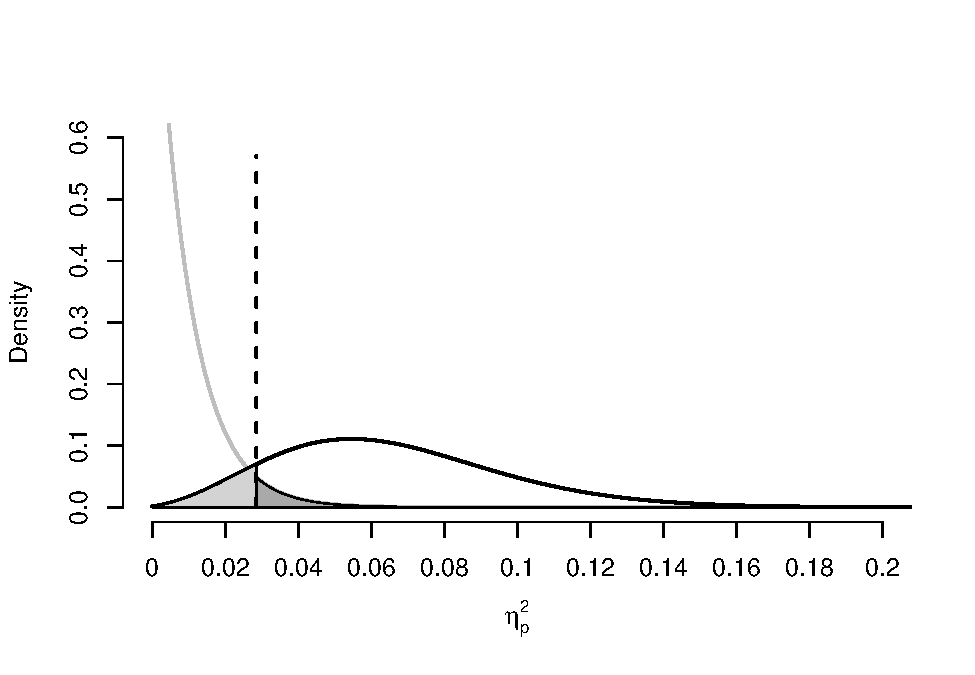
\includegraphics{1.2_validation_power_between_1x3_files/figure-latex/unnamed-chunk-1-1.pdf}

\begin{Shaded}
\begin{Highlighting}[]
\NormalTok{alpha_level <-}\StringTok{ }\FloatTok{0.05}
\CommentTok{# You should think carefully about how to justify your alpha level.}
\CommentTok{# We will give some examples later, but for now, use 0.05.}

\KeywordTok{ANOVA_power}\NormalTok{(design_result, }\DataTypeTok{alpha_level =}\NormalTok{ alpha_level, }\DataTypeTok{nsims =}\NormalTok{ nsims)}
\end{Highlighting}
\end{Shaded}

\begin{verbatim}
## Power and Effect sizes for ANOVA tests
##                  power effect size
## anova_condition 47.761      0.0383
## 
## Power and Effect sizes for contrasts
##                                    power effect size
## p_condition_control_condition_cat 39.847      0.3466
## p_condition_control_condition_dog 52.285      0.4103
## p_condition_cat_condition_dog      6.034      0.0637
\end{verbatim}

\begin{Shaded}
\begin{Highlighting}[]
\CommentTok{#should yield}
\CommentTok{#0.3983064}
\CommentTok{#0.5205162}
\CommentTok{#0.06104044}
\end{Highlighting}
\end{Shaded}

The result shows that you would have quite low power with 50
participants, both for the overall ANOVA (just around 50\% power), as
for the follow up comparisons (approximately 40\% power for the control
vs cat condition, around 50\% for the control vs dogs condition, and a
really low power (around 6\%, just above the Type 1 error rate of 5\%)
for the expected difference between cats and dogs.

\subsection{Power for simple effects}\label{power-for-simple-effects}

We are typically not just interested in the ANOVA, but also in follow up
comparisons. In this case, we would perform a \emph{t}-test comparing
the control condition against the cat and dog condition, and we would
compare the cat and dog conditions against each other, in independent
\emph{t}-tests.

For our example, Cohen's d (the standardized mean difference) is
2.2/6.4, or d = 0.34375 for the difference between the control condition
and cats, 2.6/6.4 of d = 0.40625 for the difference between the control
condition and dogs, and 0.4/6.4 or d = 0.0625 for the difference between
cats and dogs as pets.

We can easily compute the expected power for these simple comparisons
using the pwr package.

\begin{Shaded}
\begin{Highlighting}[]
\KeywordTok{pwr.t.test}\NormalTok{(}\DataTypeTok{d =} \FloatTok{2.2}\OperatorTok{/}\FloatTok{6.4}\NormalTok{,}
           \DataTypeTok{n =} \DecValTok{50}\NormalTok{,}
           \DataTypeTok{sig.level =} \FloatTok{0.05}\NormalTok{,}
           \DataTypeTok{type=}\StringTok{"two.sample"}\NormalTok{,}
           \DataTypeTok{alternative=}\StringTok{"two.sided"}\NormalTok{)}\OperatorTok{$}\NormalTok{power}
\end{Highlighting}
\end{Shaded}

\begin{verbatim}
## [1] 0.3983064
\end{verbatim}

\begin{Shaded}
\begin{Highlighting}[]
\KeywordTok{pwr.t.test}\NormalTok{(}\DataTypeTok{d =} \FloatTok{2.6}\OperatorTok{/}\FloatTok{6.4}\NormalTok{,}
           \DataTypeTok{n =} \DecValTok{50}\NormalTok{,}
           \DataTypeTok{sig.level =} \FloatTok{0.05}\NormalTok{,}
           \DataTypeTok{type=}\StringTok{"two.sample"}\NormalTok{,}
           \DataTypeTok{alternative=}\StringTok{"two.sided"}\NormalTok{)}\OperatorTok{$}\NormalTok{power}
\end{Highlighting}
\end{Shaded}

\begin{verbatim}
## [1] 0.5205162
\end{verbatim}

\begin{Shaded}
\begin{Highlighting}[]
\KeywordTok{pwr.t.test}\NormalTok{(}\DataTypeTok{d =} \FloatTok{0.4}\OperatorTok{/}\FloatTok{6.4}\NormalTok{,}
           \DataTypeTok{n =} \DecValTok{50}\NormalTok{,}
           \DataTypeTok{sig.level =} \FloatTok{0.05}\NormalTok{,}
           \DataTypeTok{type=}\StringTok{"two.sample"}\NormalTok{,}
           \DataTypeTok{alternative=}\StringTok{"two.sided"}\NormalTok{)}\OperatorTok{$}\NormalTok{power}
\end{Highlighting}
\end{Shaded}

\begin{verbatim}
## [1] 0.06104044
\end{verbatim}

This analysis tells us that running the study with 50 participants in
each condition is more likely to \emph{not} yield a significant test
result, even if our expected pattern of differences is true, than that
we will observe a \emph{p}-value smaller than our alpha level. This is
not optimal.

Let's mathematically explore which pattern of means we would need to
expect to habe 90\% power for the ANOVA with 50 participants in each
group. We can use the pwr package in R to compute a sensitivity analysis
that tells us the effect size, in Cohen's f, that we are able to detect
with 3 groups and 50 partiicpants in each group, in order to achive 90\%
power with an alpha level of 5\%.

\begin{Shaded}
\begin{Highlighting}[]
\NormalTok{K <-}\StringTok{ }\DecValTok{3}
\NormalTok{n <-}\StringTok{ }\DecValTok{50}
\NormalTok{sd <-}\StringTok{ }\FloatTok{6.4}
\NormalTok{r <-}\StringTok{ }\DecValTok{0}

\CommentTok{#Calculate f when running simulation}
\NormalTok{f <-}\StringTok{ }\KeywordTok{pwr.anova.test}\NormalTok{(}\DataTypeTok{n =}\NormalTok{ n,}
                    \DataTypeTok{k =}\NormalTok{ K,}
                    \DataTypeTok{power =} \FloatTok{0.9}\NormalTok{,}
                    \DataTypeTok{sig.level =}\NormalTok{ alpha_level)}\OperatorTok{$}\NormalTok{f}
\NormalTok{f}
\end{Highlighting}
\end{Shaded}

\begin{verbatim}
## [1] 0.2934417
\end{verbatim}

This sensitivity analysis shows we have 90\% power in our planned design
to detect effects of Cohen's f of 0.2934417. Benchmarks by Cohen (1988)
for small, medium, and large Cohen's f values are 0.1, 0.25, and 0.4,
which correspond to eta-squared values of small (.0099), medium (.0588),
and large (.1379), in line with d = .2, .5, or .8. So, at least based on
these benchmarks, we have 90\% power to detect effects that are somewhat
sizeable.

\begin{Shaded}
\begin{Highlighting}[]
\NormalTok{f2 <-}\StringTok{ }\NormalTok{f}\OperatorTok{^}\DecValTok{2}
\NormalTok{ES <-}\StringTok{ }\NormalTok{f2}\OperatorTok{/}\NormalTok{(f2}\OperatorTok{+}\DecValTok{1}\NormalTok{)}
\NormalTok{ES}
\end{Highlighting}
\end{Shaded}

\begin{verbatim}
## [1] 0.07928127
\end{verbatim}

Expressed in eta-squared, we can detect values of eta-squared = 0.0793
or larger.

\begin{Shaded}
\begin{Highlighting}[]
\NormalTok{mu <-}\StringTok{ }\KeywordTok{mu_from_ES}\NormalTok{(}\DataTypeTok{K =}\NormalTok{ K, }\DataTypeTok{ES =}\NormalTok{ ES)}
\NormalTok{mu <-}\StringTok{ }\NormalTok{mu }\OperatorTok{*}\StringTok{ }\NormalTok{sd}
\NormalTok{mu}
\end{Highlighting}
\end{Shaded}

\begin{verbatim}
## [1] -2.300104  0.000000  2.300104
\end{verbatim}

We can compute a pattern of means, given a standard deviation of 6.4,
that would give us an effect size of f = 0.2934, or eta-squared of
0.0793. We should be able to accomplish this is the means are -2.300104,
0.000000, and 2.300104. We can use these values to confirm the ANOVA has
90\% power.

\begin{Shaded}
\begin{Highlighting}[]
\NormalTok{design_result <-}\StringTok{ }\KeywordTok{ANOVA_design}\NormalTok{(}\DataTypeTok{string =}\NormalTok{ string,}
                   \DataTypeTok{n =}\NormalTok{ n, }
                   \DataTypeTok{mu =}\NormalTok{ mu, }
                   \DataTypeTok{sd =}\NormalTok{ sd, }
                   \DataTypeTok{labelnames =}\NormalTok{ labelnames)}
\end{Highlighting}
\end{Shaded}

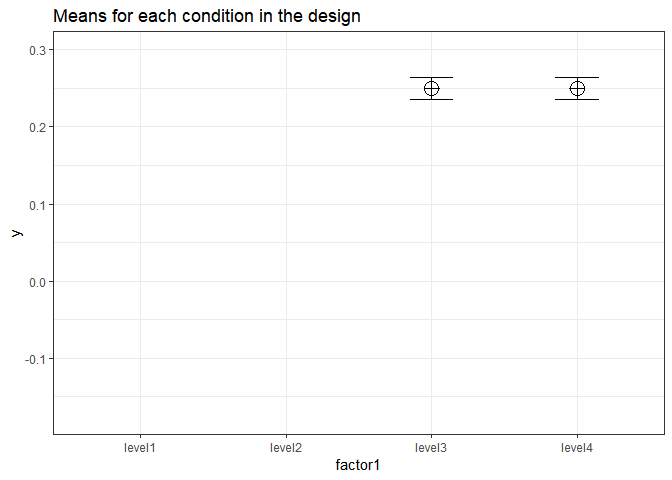
\includegraphics{1.2_validation_power_between_1x3_files/figure-latex/unnamed-chunk-6-1.pdf}

\begin{Shaded}
\begin{Highlighting}[]
\KeywordTok{ANOVA_power}\NormalTok{(design_result, }\DataTypeTok{alpha_level =}\NormalTok{ alpha_level, }\DataTypeTok{nsims =}\NormalTok{ nsims)}
\end{Highlighting}
\end{Shaded}

\begin{verbatim}
## Power and Effect sizes for ANOVA tests
##                  power effect size
## anova_condition 89.986      0.0867
## 
## Power and Effect sizes for contrasts
##                                    power effect size
## p_condition_control_condition_cat 42.686      0.3622
## p_condition_control_condition_dog 94.507      0.7239
## p_condition_cat_condition_dog     42.674      0.3615
\end{verbatim}

The simulation confirms that for the \emph{F}-test for the ANOVA we have
90\% power. This is also what g*power tells us what would happen based
on a post-hoc power analysis with an f of 0.2934417, 3 groups, 150
participants in total (50 in each between subject condition), and an
alpha of 5\%.

\begin{figure}
\centering
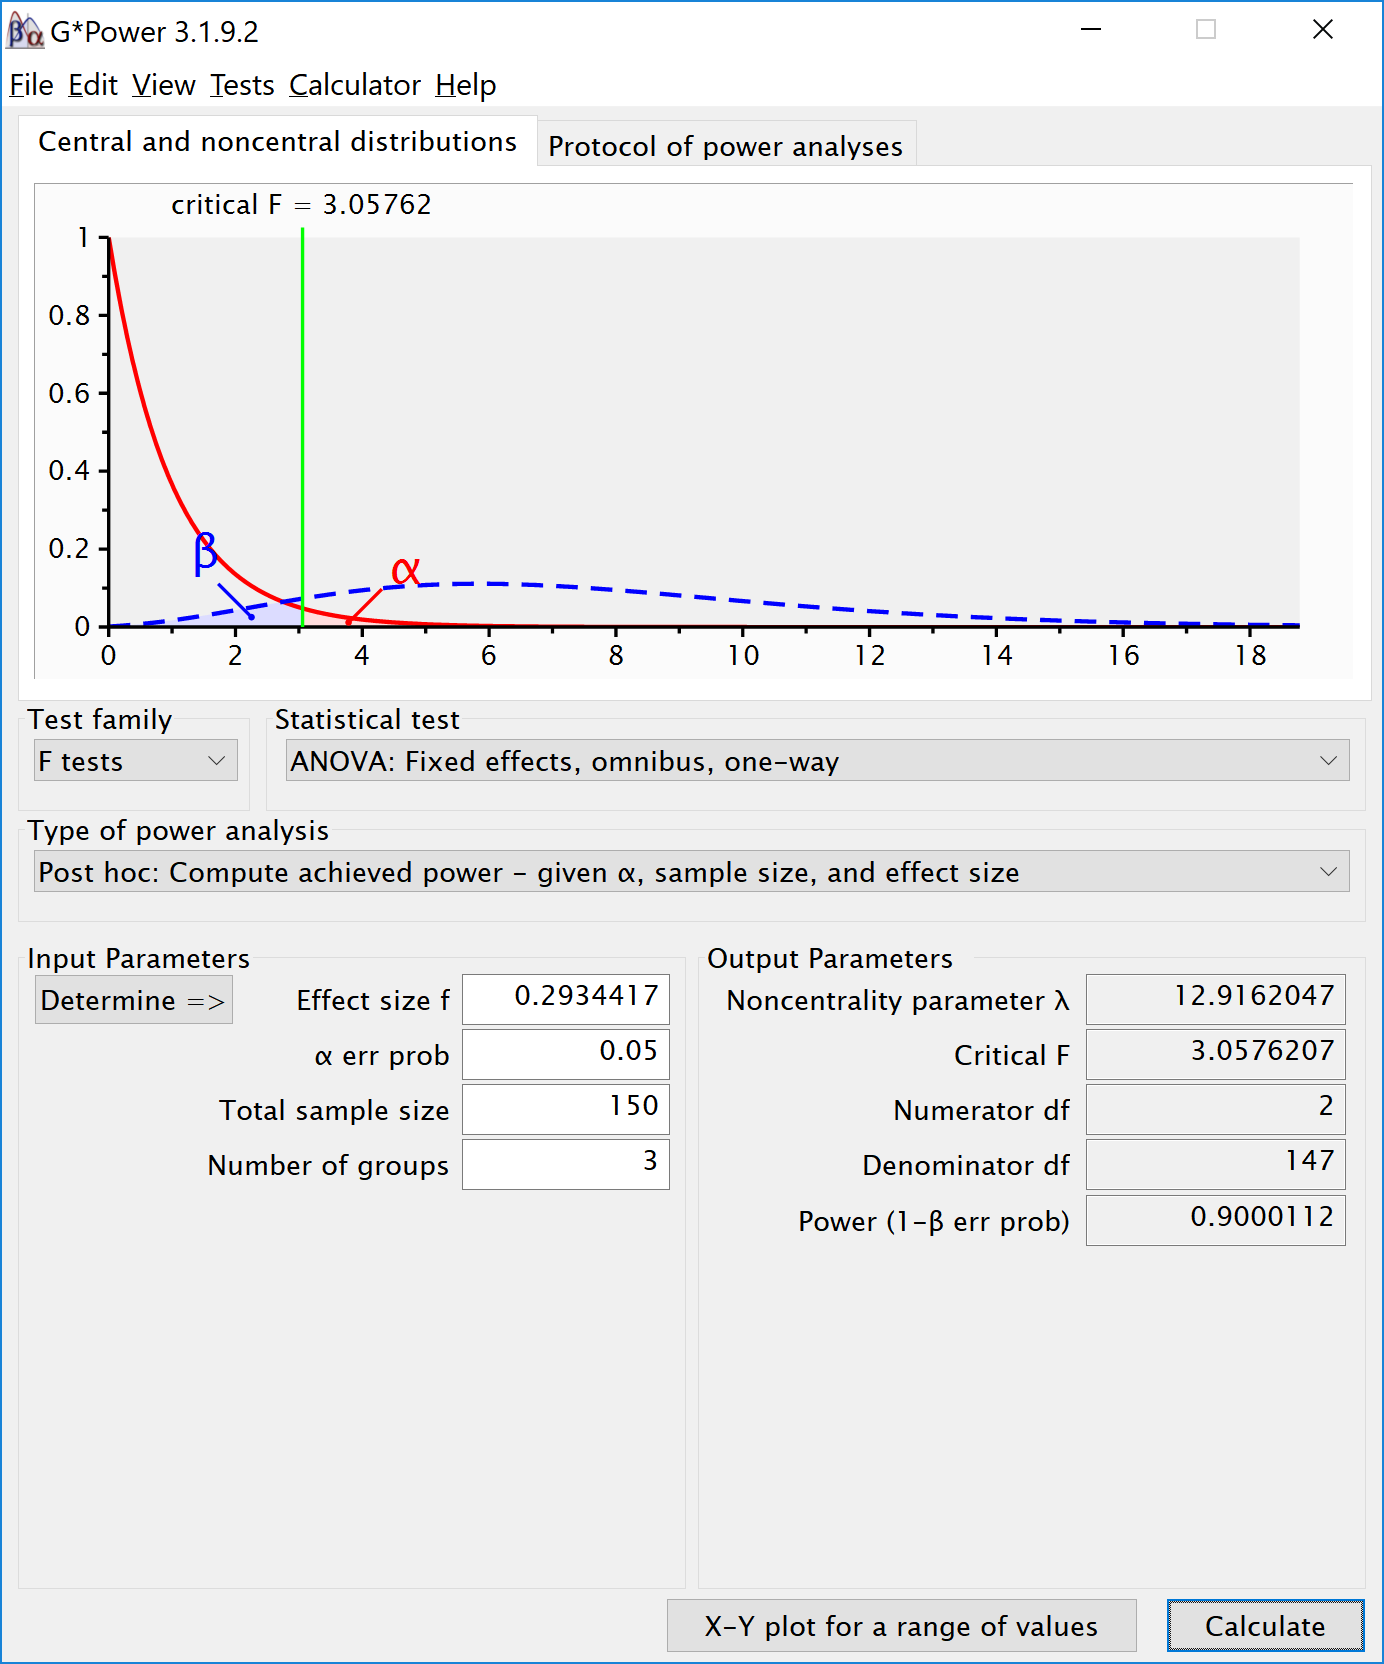
\includegraphics{screenshots/gpower_7.png}
\caption{}
\end{figure}

We can also compute the power for the ANOVA and simple effects in R with
the pwr package. The calculated effect sizes and power match those from
the simulation.

\begin{Shaded}
\begin{Highlighting}[]
\NormalTok{K <-}\StringTok{ }\DecValTok{3}
\NormalTok{n <-}\StringTok{ }\DecValTok{50}
\NormalTok{sd <-}\StringTok{ }\FloatTok{6.4}
\NormalTok{f <-}\StringTok{ }\FloatTok{0.2934417}

\KeywordTok{pwr.anova.test}\NormalTok{(}\DataTypeTok{n =}\NormalTok{ n,}
               \DataTypeTok{k =}\NormalTok{ K,}
               \DataTypeTok{f =}\NormalTok{ f,}
               \DataTypeTok{sig.level =}\NormalTok{ alpha_level)}\OperatorTok{$}\NormalTok{power}
\end{Highlighting}
\end{Shaded}

\begin{verbatim}
## [1] 0.9000112
\end{verbatim}

\begin{Shaded}
\begin{Highlighting}[]
\NormalTok{d <-}\StringTok{ }\FloatTok{2.300104}\OperatorTok{/}\FloatTok{6.4}
\NormalTok{d}
\end{Highlighting}
\end{Shaded}

\begin{verbatim}
## [1] 0.3593912
\end{verbatim}

\begin{Shaded}
\begin{Highlighting}[]
\KeywordTok{pwr.t.test}\NormalTok{(}\DataTypeTok{d =} \FloatTok{2.300104}\OperatorTok{/}\FloatTok{6.4}\NormalTok{,}
           \DataTypeTok{n =} \DecValTok{50}\NormalTok{,}
           \DataTypeTok{sig.level =} \FloatTok{0.05}\NormalTok{,}
           \DataTypeTok{type=}\StringTok{"two.sample"}\NormalTok{,}
           \DataTypeTok{alternative=}\StringTok{"two.sided"}\NormalTok{)}\OperatorTok{$}\NormalTok{power}
\end{Highlighting}
\end{Shaded}

\begin{verbatim}
## [1] 0.4284243
\end{verbatim}

\begin{Shaded}
\begin{Highlighting}[]
\NormalTok{d <-}\StringTok{ }\DecValTok{2}\OperatorTok{*}\FloatTok{2.300104}\OperatorTok{/}\FloatTok{6.4}
\NormalTok{d}
\end{Highlighting}
\end{Shaded}

\begin{verbatim}
## [1] 0.7187825
\end{verbatim}

\begin{Shaded}
\begin{Highlighting}[]
\KeywordTok{pwr.t.test}\NormalTok{(}\DataTypeTok{d =}\NormalTok{ d,}
           \DataTypeTok{n =} \DecValTok{50}\NormalTok{,}
           \DataTypeTok{sig.level =} \FloatTok{0.05}\NormalTok{,}
           \DataTypeTok{type=}\StringTok{"two.sample"}\NormalTok{,}
           \DataTypeTok{alternative=}\StringTok{"two.sided"}\NormalTok{)}\OperatorTok{$}\NormalTok{power}
\end{Highlighting}
\end{Shaded}

\begin{verbatim}
## [1] 0.9450353
\end{verbatim}

We can also compare the results against the analytic solution by Aberson
(2019).

First, load the function for a 3-way ANOVA.

\begin{Shaded}
\begin{Highlighting}[]
\NormalTok{anova1f_}\DecValTok{3}\NormalTok{<-}\ControlFlowTok{function}\NormalTok{(}\DataTypeTok{m1=}\OtherTok{NULL}\NormalTok{,}\DataTypeTok{m2=}\OtherTok{NULL}\NormalTok{,}\DataTypeTok{m3=}\OtherTok{NULL}\NormalTok{,}\DataTypeTok{s1=}\OtherTok{NULL}\NormalTok{,}\DataTypeTok{s2=}\OtherTok{NULL}\NormalTok{,}\DataTypeTok{s3=}\OtherTok{NULL}\NormalTok{,}\DataTypeTok{n1=}\OtherTok{NULL}\NormalTok{,}\DataTypeTok{n2=}\OtherTok{NULL}\NormalTok{,}\DataTypeTok{n3=}\OtherTok{NULL}\NormalTok{,}\DataTypeTok{alpha=}\NormalTok{.}\DecValTok{05}\NormalTok{)\{}
\NormalTok{x<-stats}\OperatorTok{::}\KeywordTok{rnorm}\NormalTok{(n1,m1,s1)}
\NormalTok{X<-x}
\NormalTok{MEAN<-m1}
\NormalTok{SD<-s1}
\NormalTok{Z <-}\StringTok{ }\NormalTok{(((X }\OperatorTok{-}\StringTok{ }\KeywordTok{mean}\NormalTok{(X, }\DataTypeTok{na.rm =} \OtherTok{TRUE}\NormalTok{))}\OperatorTok{/}\NormalTok{stats}\OperatorTok{::}\KeywordTok{sd}\NormalTok{(X, }\DataTypeTok{na.rm =} \OtherTok{TRUE}\NormalTok{))) }\OperatorTok{*}\StringTok{ }\NormalTok{SD}
\NormalTok{y<-MEAN }\OperatorTok{+}\StringTok{ }\NormalTok{Z}
\NormalTok{group<-}\KeywordTok{rep}\NormalTok{(}\StringTok{"A1"}\NormalTok{,n1)}
\NormalTok{l1<-}\KeywordTok{data.frame}\NormalTok{(y, group)}
\NormalTok{x<-stats}\OperatorTok{::}\KeywordTok{rnorm}\NormalTok{(n2,m2,s2)}
\NormalTok{X<-x}
\NormalTok{MEAN<-m2}
\NormalTok{SD<-s2}
\NormalTok{Z <-}\StringTok{ }\NormalTok{(((X }\OperatorTok{-}\StringTok{ }\KeywordTok{mean}\NormalTok{(X, }\DataTypeTok{na.rm =} \OtherTok{TRUE}\NormalTok{))}\OperatorTok{/}\NormalTok{stats}\OperatorTok{::}\KeywordTok{sd}\NormalTok{(X, }\DataTypeTok{na.rm =} \OtherTok{TRUE}\NormalTok{))) }\OperatorTok{*}\StringTok{ }\NormalTok{SD}
\NormalTok{y<-MEAN }\OperatorTok{+}\StringTok{ }\NormalTok{Z}
\NormalTok{group<-}\KeywordTok{rep}\NormalTok{(}\StringTok{"A2"}\NormalTok{,n2)}
\NormalTok{l2<-}\KeywordTok{data.frame}\NormalTok{(y, group)}
\NormalTok{x<-stats}\OperatorTok{::}\KeywordTok{rnorm}\NormalTok{(n3,m3,s3)}
\NormalTok{X<-x}
\NormalTok{MEAN<-m3}
\NormalTok{SD<-s3}
\NormalTok{Z <-}\StringTok{ }\NormalTok{(((X }\OperatorTok{-}\StringTok{ }\KeywordTok{mean}\NormalTok{(X, }\DataTypeTok{na.rm =} \OtherTok{TRUE}\NormalTok{))}\OperatorTok{/}\NormalTok{stats}\OperatorTok{::}\KeywordTok{sd}\NormalTok{(X, }\DataTypeTok{na.rm =} \OtherTok{TRUE}\NormalTok{))) }\OperatorTok{*}\StringTok{ }\NormalTok{SD}
\NormalTok{y<-MEAN }\OperatorTok{+}\StringTok{ }\NormalTok{Z}
\NormalTok{group<-}\KeywordTok{rep}\NormalTok{(}\StringTok{"A3"}\NormalTok{,n3)}
\NormalTok{l3<-}\KeywordTok{data.frame}\NormalTok{(y, group)}
\NormalTok{simdat<-}\KeywordTok{rbind}\NormalTok{(l1,l2,l3)}
\NormalTok{anova<-stats}\OperatorTok{::}\KeywordTok{aov}\NormalTok{(y}\OperatorTok{~}\NormalTok{group, }\DataTypeTok{data=}\NormalTok{simdat)}
\NormalTok{anova<-car}\OperatorTok{::}\KeywordTok{Anova}\NormalTok{(anova, }\DataTypeTok{type=}\StringTok{"III"}\NormalTok{)}
\NormalTok{SSA<-anova[}\DecValTok{2}\NormalTok{,}\DecValTok{1}\NormalTok{] }\CommentTok{#column, row}
\NormalTok{SSwin<-anova[}\DecValTok{3}\NormalTok{,}\DecValTok{1}\NormalTok{]}
\NormalTok{dfwin<-anova[}\DecValTok{3}\NormalTok{,}\DecValTok{2}\NormalTok{]}
\NormalTok{dfbg<-anova[}\DecValTok{2}\NormalTok{,}\DecValTok{2}\NormalTok{]}
\NormalTok{eta2<-SSA}\OperatorTok{/}\NormalTok{(SSA}\OperatorTok{+}\NormalTok{SSwin)}
\NormalTok{f2<-eta2}\OperatorTok{/}\NormalTok{(}\DecValTok{1}\OperatorTok{-}\NormalTok{eta2)}
\NormalTok{lambda<-f2}\OperatorTok{*}\NormalTok{dfwin}
\NormalTok{minusalpha<-}\DecValTok{1}\OperatorTok{-}\NormalTok{alpha}
\NormalTok{Ft<-stats}\OperatorTok{::}\KeywordTok{qf}\NormalTok{(minusalpha, dfbg, dfwin)}
\NormalTok{power<-}\DecValTok{1}\OperatorTok{-}\NormalTok{stats}\OperatorTok{::}\KeywordTok{pf}\NormalTok{(Ft, dfbg,dfwin,lambda)}
\KeywordTok{list}\NormalTok{(}\DataTypeTok{Power =}\NormalTok{ power)\}}
\end{Highlighting}
\end{Shaded}

Then we use the function to calculate power.

\begin{Shaded}
\begin{Highlighting}[]
\CommentTok{#Initial example, low power}
\KeywordTok{anova1f_3}\NormalTok{(}\DataTypeTok{m1=}\DecValTok{24}\NormalTok{, }\DataTypeTok{m2=}\FloatTok{26.2}\NormalTok{, }\DataTypeTok{m3=}\FloatTok{26.6}\NormalTok{, }\DataTypeTok{s1=}\FloatTok{6.4}\NormalTok{, }\DataTypeTok{s2=}\FloatTok{6.4}\NormalTok{, }\DataTypeTok{s3=}\FloatTok{6.4}\NormalTok{, }\DataTypeTok{n1=}\DecValTok{50}\NormalTok{, }\DataTypeTok{n2=}\DecValTok{50}\NormalTok{, }\DataTypeTok{n3=}\DecValTok{50}\NormalTok{, }\DataTypeTok{alpha=}\NormalTok{.}\DecValTok{05}\NormalTok{)}
\end{Highlighting}
\end{Shaded}

\begin{verbatim}
## $Power
## [1] 0.4769468
\end{verbatim}

\begin{Shaded}
\begin{Highlighting}[]
\CommentTok{#From: Aberson, Christopher L. Applied Power Analysis for the Behavioral Sciences, 2nd Edition. }
\CommentTok{# $Power [1] 0.4769468}

\CommentTok{#Later example, based on larger mean difference}
\KeywordTok{anova1f_3}\NormalTok{(}\DataTypeTok{m1=}\OperatorTok{-}\FloatTok{2.300104}\NormalTok{, }\DataTypeTok{m2=}\DecValTok{0}\NormalTok{, }\DataTypeTok{m3=}\FloatTok{2.300104}\NormalTok{, }\DataTypeTok{s1=}\FloatTok{6.4}\NormalTok{, }\DataTypeTok{s2=}\FloatTok{6.4}\NormalTok{, }\DataTypeTok{s3=}\FloatTok{6.4}\NormalTok{, }\DataTypeTok{n1=}\DecValTok{50}\NormalTok{, }\DataTypeTok{n2=}\DecValTok{50}\NormalTok{, }\DataTypeTok{n3=}\DecValTok{50}\NormalTok{, }\DataTypeTok{alpha=}\NormalTok{.}\DecValTok{05}\NormalTok{)}
\end{Highlighting}
\end{Shaded}

\begin{verbatim}
## $Power
## [1] 0.9000112
\end{verbatim}

\begin{Shaded}
\begin{Highlighting}[]
\CommentTok{# $Power [1] 0.9000112}
\end{Highlighting}
\end{Shaded}


\end{document}
